\documentclass[aspectratio=169,spanish,xcolor=table]{beamer}
\usepackage{iftex}
\ifPDFTeX
  \usepackage[utf8]{inputenc}
  \usepackage[T1]{fontenc}
\fi
\usepackage[spanish,es-tabla,es-noshorthands]{babel}
\usepackage{helvet}
\renewcommand{\familydefault}{\sfdefault}
\usepackage{tikz,pgfplots,array,booktabs,ragged2e}
\pgfplotsset{compat=1.18}
\usetikzlibrary{arrows.meta,positioning,calc,shapes.geometric,fit}

\definecolor{iiiepeNavy}{HTML}{163B5C}
\definecolor{iiiepeBlue}{HTML}{1F6F9F}
\definecolor{iiiepeAqua}{HTML}{20B7A8}
\definecolor{iiiepeOrange}{HTML}{F28C28}
\definecolor{iiiepePaper}{HTML}{F6F8F7}
\definecolor{iiiepeInk}{HTML}{1E2A32}
\definecolor{iiiepePale}{HTML}{EEF5F8}
\definecolor{iiiepeMint}{HTML}{E7F6F4}
\definecolor{iiiepeWarm}{HTML}{FFF3E6}

\usetheme{default}
\usecolortheme{default}
\setbeamertemplate{navigation symbols}{}
\setbeamercolor{normal text}{fg=iiiepeInk,bg=white}
\setbeamercolor{structure}{fg=iiiepeNavy}
\setbeamercolor{frametitle}{fg=white,bg=iiiepeNavy}
\setbeamercolor{block title}{fg=white,bg=iiiepeBlue}
\setbeamercolor{block body}{fg=iiiepeInk,bg=iiiepePale}
\setbeamercolor{item}{fg=iiiepeOrange}

\setbeamertemplate{frametitle}{%
  \nointerlineskip%
  \begin{beamercolorbox}[wd=\paperwidth,ht=0.95cm,dp=0.22cm,leftskip=0.45cm,rightskip=0.45cm]{frametitle}%
    \begin{minipage}[c]{13.2cm}\usebeamerfont{frametitle}\large\bfseries\insertframetitle\end{minipage}%
    \hfill\begin{minipage}[c]{1.6cm}\raggedleft\includegraphics[height=0.56cm]{img/iiiepe/logo-iiiepe-blanco.png}\end{minipage}%
  \end{beamercolorbox}%
}

\setbeamertemplate{footline}{%
  \leavevmode%
  \hbox{%
    \begin{beamercolorbox}[wd=.78\paperwidth,ht=0.5cm,dp=0.18cm,leftskip=0.45cm]{frametitle}%
      \scriptsize\color{white}M. de la Cruz Muñoz · MAEM · Matrícula 00874 · SD26 · Actividad 3 · Infografía%
    \end{beamercolorbox}%
    \begin{beamercolorbox}[wd=.22\paperwidth,ht=0.5cm,dp=0.18cm,rightskip=0.45cm]{frametitle}%
      \hfill\scriptsize\color{white}\insertframenumber{} / \inserttotalframenumber%
    \end{beamercolorbox}%
  }%
  \vskip0pt%
}

\newcommand{\Pill}[2]{%
  \tikz[baseline=(x.base)]{\node[rounded corners=3pt,fill=#1!14,draw=#1!75!black,thick,inner xsep=6pt,inner ysep=4pt,align=center] (x) {\scriptsize\bfseries #2};}%
}

\title{Infografía Crítica: Philippe Meirieu (2020) y Tres Miradas de Sesión 3}
\subtitle{Actividad 3 · Módulo 51440 · LaTeX/TikZ}
\author{Mtro. Martín Jonathan de la Cruz Muñoz · Matrícula 00874}
\institute{IIIEPE · Maestría en Aprendizaje y Enseñanza de las Matemáticas · Grupo A}
\date{19 de noviembre de 2026}

% Motor visual editorial para infografías en LaTeX/TikZ (Cohorte SD26 · IIIEPE MAEM)
\definecolor{infNavy}{HTML}{1A4F7A}
\definecolor{infBlueLight}{HTML}{DCEBF7}
\definecolor{infBlueCard}{HTML}{EDF5FC}
\definecolor{infBlueAccent}{HTML}{2775B3}

\definecolor{infGreen}{HTML}{1E6B43}
\definecolor{infGreenLight}{HTML}{DCF2E4}
\definecolor{infGreenCard}{HTML}{EEF9F2}
\definecolor{infGreenAccent}{HTML}{2A935B}

\definecolor{infOrange}{HTML}{C45522}
\definecolor{infOrangeLight}{HTML}{FDE6D8}
\definecolor{infOrangeCard}{HTML}{FEF3EB}
\definecolor{infOrangeAccent}{HTML}{DE6A31}

\definecolor{infInk}{HTML}{1E2932}
\definecolor{infPaper}{HTML}{F8FAFC}
\definecolor{infBorder}{HTML}{C9D6E2}

\tikzset{
  pics/inf_target/.style={code={
    \draw (0,0) circle (.78);
    \draw (0,0) circle (.46);
    \fill (0,0) circle (.16);
    \draw[line width=1.4pt] (.42,.42) -- (.95,.95);
    \draw (.62,.95) -- (.95,.95) -- (.95,.62);
  }},
  pics/inf_doc/.style={code={
    \draw[rounded corners=1.2pt] (-.65,-.85) rectangle (.65,.85);
    \draw (-.38,.42) -- (.38,.42);
    \draw (-.38,.08) -- (.38,.08);
    \draw (-.38,-.26) -- (.38,-.26);
    \draw (-.38,-.58) -- (.12,-.58);
  }},
  pics/inf_key/.style={code={
    \draw (-.38,.12) circle (.38);
    \draw[line width=1.6pt] (0,.12) -- (.92,.12);
    \draw[line width=1.5pt] (.58,.12) -- (.58,-.28);
    \draw[line width=1.5pt] (.85,.12) -- (.85,-.20);
  }},
  pics/inf_bulb/.style={code={
    \draw (-.32,-.28) .. controls (-.58,-.05) and (-.62,.45) .. (0,.65)
      .. controls (.62,.45) and (.58,-.05) .. (.32,-.28) -- cycle;
    \draw (-.26,-.48) -- (.26,-.48);
    \draw (-.20,-.70) -- (.20,-.70);
    \draw (0,.82) -- (0,1.02) (.68,.55) -- (.84,.68) (-.68,.55) -- (-.84,.68);
  }},
  pics/inf_gear/.style={code={
    \draw (0,0) circle (.46);
    \draw (0,0) circle (.18);
    \foreach \a in {0,45,...,315}{
      \draw[line width=2.2pt] (\a:.46) -- (\a:.76);
    }
  }},
  pics/inf_personas/.style={code={
    \draw (0,.48) circle (.24);
    \draw (-.64,.25) circle (.19) (.64,.25) circle (.19);
    \draw (-.42,-.72) -- (-.42,-.18) .. controls (-.42,.18) and (.42,.18) .. (.42,-.18) -- (.42,-.72);
    \draw (-.95,-.66) -- (-.95,-.24) .. controls (-.95,.02) and (-.56,.02) .. (-.48,-.22);
    \draw (.48,-.22) .. controls (.56,.02) and (.95,.02) .. (.95,-.24) -- (.95,-.66);
  }},
  pics/inf_autonomia/.style={code={
    \draw[dashed] (0,0) circle (.88);
    \draw (0,.42) circle (.24);
    \draw (-.38,-.58) -- (-.38,-.15) .. controls (-.38,.18) and (.38,.18) .. (.38,-.15) -- (.38,-.58);
  }},
  pics/inf_alerta/.style={code={
    \draw[rounded corners=1.5pt] (0,.85) -- (-.92,-.72) -- (.92,-.72) -- cycle;
    \draw[line width=1.6pt] (0,.30) -- (0,-.22);
    \fill (0,-.48) circle (.09);
  }},
  pics/inf_balanza/.style={code={
    \draw (0,-.75) -- (0,.72);
    \draw (-.50,-.75) -- (.50,-.75);
    \draw (-.75,.48) -- (.75,.48);
    \draw (-.75,.48) -- (-.95,-.05) -- (-.55,-.05) -- cycle;
    \draw (.75,.48) -- (.55,-.05) -- (.95,-.05) -- cycle;
  }},
  pics/inf_cerebro/.style={code={
    \draw (-.1,.62) .. controls (-.72,.68) and (-.95,.15) .. (-.68,-.28)
      .. controls (-.82,-.65) and (-.28,-.75) .. (0,-.52);
    \draw (.1,.62) .. controls (.72,.68) and (.95,.15) .. (.68,-.28)
      .. controls (.82,-.65) and (.28,-.75) .. (0,-.52);
    \draw (0,.65) -- (0,-.52);
    \draw (-.45,.18) -- (-.15,.05) (.45,.18) -- (.15,.05) (-.42,-.22) -- (-.12,-.18);
  }},
  pics/inf_construccion/.style={code={
    \draw (0,0) circle (.45);
    \draw (0,0) circle (.16);
    \foreach \a in {0,60,...,300}{
      \draw[line width=2pt] (\a:.45) -- (\a:.74);
    }
    \draw (.62,.62) circle (.22);
  }},
  pics/inf_dialogo/.style={code={
    \draw[rounded corners=2pt] (-.92,.78) -- (.48,.78) -- (.48,-.04)
      -- (-.32,-.04) -- (-.68,-.40) -- (-.68,-.04) -- (-.92,-.04) -- cycle;
    \draw[rounded corners=1.5pt] (.15,-.18) -- (.92,-.18) -- (.92,-.76)
      -- (.68,-.76) -- (.68,-.98) -- (.38,-.76) -- (.15,-.76) -- cycle;
    \draw (-.64,.48) -- (.22,.48) (-.64,.22) -- (.06,.22);
  }},
  pics/inf_grafica/.style={code={
    \draw (-.88,.85) -- (-.88,-.75) -- (.92,-.75);
    \fill (-.62,-.75) rectangle (-.32,-.10);
    \fill (-.15,-.75) rectangle (.15,.25);
    \fill (.32,-.75) rectangle (.62,.68);
  }},
  pics/inf_lupa/.style={code={
    \draw (-.18,.22) circle (.54);
    \draw[line width=1.8pt] (.22,-.18) -- (.88,-.84);
    \draw (-.48,.28) .. controls (-.44,.50) and (-.26,.58) .. (-.06,.56);
  }},
  pics/inf_escuela/.style={code={
    \draw (-.85,-.75) rectangle (.85,.25);
    \draw (-1.0,.25) -- (0,.92) -- (1.0,.25);
    \draw (-.20,-.75) rectangle (.20,-.10);
    \draw (-.64,-.08) rectangle (-.38,.12);
    \draw (.38,-.08) rectangle (.64,.12);
    \draw (0,.52) circle (.12);
  }},
  pics/inf_andamio/.style={code={
    \draw (-.82,-.75) -- (-.82,.75) (.82,-.75) -- (.82,.75);
    \draw (-.82,-.30) -- (.82,-.30) (-.82,.22) -- (.82,.22) (-.82,.72) -- (.82,.72);
    \draw (-.82,-.30) -- (.82,.22) (.82,-.30) -- (-.82,.22);
    \fill[draw=none] (0,.84) circle (.10);
  }},
  pics/inf_libro/.style={code={
    \draw (0,-.68) -- (0,.58);
    \draw (0,.58) .. controls (-.34,.85) and (-.68,.85) .. (-.96,.64)
      -- (-.96,-.58) .. controls (-.58,-.42) and (-.26,-.45) .. (0,-.68);
    \draw (0,.58) .. controls (.34,.85) and (.68,.85) .. (.96,.64)
      -- (.96,-.58) .. controls (.58,-.42) and (.26,-.45) .. (0,-.68);
    \draw (-.72,.28) -- (-.24,.14) (-.72,-.04) -- (-.24,-.18);
    \draw (.24,.14) -- (.72,.28) (.24,-.18) -- (.72,-.04);
  }}
}

\newcommand{\InfIcon}[3][0.30]{%
  \begin{tikzpicture}[x=#1cm,y=#1cm,baseline=-0.12cm]
    \path[use as bounding box] (-1.05,-1.05) rectangle (1.05,1.05);
    \pic[draw=#3,fill=#3,line width=1.15pt,line cap=round,line join=round] {inf_#2};
  \end{tikzpicture}%
}

\newcommand{\InfIconOutline}[3][0.30]{%
  \begin{tikzpicture}[x=#1cm,y=#1cm,baseline=-0.12cm]
    \path[use as bounding box] (-1.05,-1.05) rectangle (1.05,1.05);
    \pic[draw=#3,line width=1.15pt,line cap=round,line join=round] {inf_#2};
  \end{tikzpicture}%
}

\newcommand{\InfPillBar}[5]{%
  % #1=x, #2=y, #3=colorDark, #4=colorLight, #5=iconName, macro uses text via helper? Wait: pass #6=Title
}

% Medallón + Píldora horizontal de sección (ancho 7.75cm dentro de columna 8.15cm)
\newcommand{\InfSectionBar}[6]{%
  % (#1,#2)=origen izq, #3=accentColor, #4=lightColor, #5=icon, #6=Title
  \fill[#4,rounded corners=7pt] ({#1+0.25},{#2-0.46}) rectangle ({#1+7.75},{#2-0.02});
  \node[anchor=west,font=\fontsize{8.1}{9.5}\selectfont\bfseries\color{#3}] at ({#1+0.78},{#2-0.24}) {#6};
  \filldraw[fill=#3,draw=white,line width=1.4pt] ({#1+0.34},{#2-0.24}) circle (0.28cm);
  \node[inner sep=0pt] at ({#1+0.34},{#2-0.24}) {\InfIconOutline[0.18]{#5}{white}};
}

% Mini-tarjeta cuadrada de concepto clave (ancho 1.83cm x alto 2.18cm)
\newcommand{\InfConceptCard}[6]{%
  % #1=x, #2=y_top, #3=accentColor, #4=cardBg, #5=icon, #6=Title\\desc
  \draw[fill=#4,draw=#3!35!white,line width=0.6pt,rounded corners=4pt] ({#1},{#2-2.18}) rectangle ({#1+1.83},{#2});
  \node[inner sep=0pt] at ({#1+0.915},{#2-0.52}) {\InfIconOutline[0.32]{#5}{#3}};
  \node[anchor=north,text width=1.68cm,align=center,font=\fontsize{5.6}{6.8}\selectfont\color{infInk},inner sep=1pt] at ({#1+0.915},{#2-0.96}) {#6};
}

% Viñeta con círculo de color (Tesis / Aportes principales)
\newcommand{\InfBullet}[4]{%
  % #1=x, #2=y_top, #3=accentColor, #4=texto
  \fill[#3] ({#1+0.12},{#2-0.14}) circle (0.065cm);
  \node[anchor=north west,text width=7.35cm,align=left,font=\fontsize{6.3}{7.6}\selectfont\color{infInk},inner sep=0pt] at ({#1+0.28},{#2}) {#4};
}

% Viñeta con círculo Check ✓ (Implicaciones para la práctica)
\newcommand{\InfCheck}[4]{%
  % #1=x, #2=y_top, #3=accentColor, #4=texto
  \fill[#3] ({#1+0.14},{#2-0.15}) circle (0.125cm);
  \draw[white,line width=0.95pt,line cap=round,line join=round] ({#1+0.075},{#2-0.16}) -- ({#1+0.125},{#2-0.21}) -- ({#1+0.215},{#2-0.095});
  \node[anchor=north west,text width=7.28cm,align=left,font=\fontsize{6.3}{7.6}\selectfont\color{infInk},inner sep=0pt] at ({#1+0.34},{#2}) {#4};
}

\begin{document}

\begin{frame}[plain]
  \begin{tikzpicture}[remember picture,overlay]
    \fill[iiiepeNavy] (current page.north west) rectangle ([xshift=10.3cm]current page.south west);
    \fill[iiiepeBlue] ([xshift=10.3cm]current page.north west) rectangle (current page.south east);
    \fill[iiiepeOrange] ([xshift=0.8cm,yshift=-6.45cm]current page.north west) rectangle ([xshift=9.3cm,yshift=-6.53cm]current page.north west);
    \node[anchor=north west,text width=8.7cm,align=left] at ([xshift=0.8cm,yshift=-1.15cm]current page.north west) {%
      {\color{iiiepeAqua!45!white}\small\bfseries MAESTRÍA EN APRENDIZAJE Y ENSEÑANZA DE LAS MATEMÁTICAS · SD26\par}%
      \vspace{0.35cm}
      {\color{white}\Large\bfseries \inserttitle\par}%
      \vspace{0.25cm}
      {\color{white!90}\normalsize \insertsubtitle\par}%
    };
    \node[anchor=south west,text width=8.7cm,align=left] at ([xshift=0.8cm,yshift=0.75cm]current page.south west) {%
      {\color{white}\normalsize\bfseries Mtro. Martín Jonathan de la Cruz Muñoz\par}%
      {\color{white!85}\scriptsize Matrícula 00874 · martin.delacruz@campus.iiiepe.edu.mx\par}%
      {\color{iiiepeAqua!35!white}\scriptsize Monterrey, Nuevo León · 19 de noviembre de 2026\par}%
    };
    \node[anchor=center,text width=5.0cm,align=center] at ([xshift=13.15cm,yshift=-4.5cm]current page.north west) {%
      \includegraphics[width=3.6cm]{img/iiiepe/logo-iiiepe-blanco.png}\par\vspace{0.45cm}%
      {\color{white}\large\bfseries IIIEPE\par}%
      \vspace{0.1cm}%
      {\color{white!85}\scriptsize Fundamentos para la enseñanza\\y el aprendizaje I\par}%
    };
  \end{tikzpicture}
\end{frame}
\begin{frame}[plain]
  \centering
  \resizebox{0.97\textwidth}{!}{\begin{tikzpicture}[x=1cm,y=1cm]
  \fill[infPaper] (-0.30,-17.05) rectangle (25.45,0.20);

  % COL 1: BRECHA Y HACER ESCUELA
  \draw[fill=white,draw=infNavy,line width=1.1pt,rounded corners=7pt] (0.0,-15.72) rectangle (8.15,0.0);
  \fill[infNavy,rounded corners=6pt] (0.0,-2.48) rectangle (8.15,0.0);
  \fill[infNavy] (0.0,-2.48) rectangle (8.15,-2.00);
  \node[anchor=north west,text width=5.45cm,align=left,inner sep=0pt] at (0.28,-0.22) {%
    {\color{white}\fontsize{11.5}{13.5}\selectfont\bfseries Philippe Meirieu (I)\par}\vspace{2pt}%
    {\color{white!90}\fontsize{7.3}{8.6}\selectfont\bfseries Crisis educativa, brecha y\\sentido de «hacer escuela»\par}\vspace{3pt}%
    {\colorbox{infBlueAccent}{\color{white}\fontsize{6.3}{7.3}\selectfont\bfseries\ Eje 1 · Institución y Bien Común \ }}%
  };
  \node[inner sep=0pt] at (6.92,-1.24) {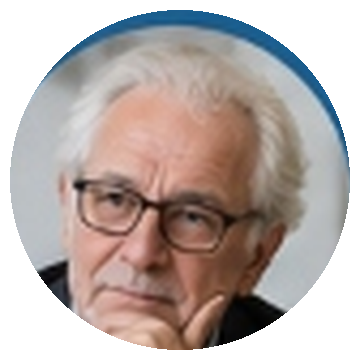
\includegraphics[width=2.06cm]{img_infografia/meirieu_photo.png}};

  \fill[infBlueLight] (0.12,-3.04) rectangle (8.03,-2.56);
  \node[font=\fontsize{6.9}{8.0}\selectfont\bfseries\color{infNavy}] at (4.075,-2.80) {«La escuela después»... ¿con la pedagogía de antes? (2020)};

  \InfSectionBar{0.20}{-3.16}{infNavy}{infBlueLight}{target}{Idea central del eje}
  \node[anchor=north west,text width=7.65cm,align=left,font=\fontsize{6.6}{8.0}\selectfont\color{infInk},inner sep=0pt] at (0.25,-3.74) {%
    Declarar «un antes y un después» es vano si el miedo y la inercia producen un «regreso a lo anormal». La escuela es institución pública donde se articula lo común y lo singular.%
  };

  \InfSectionBar{0.20}{-4.86}{infNavy}{infBlueLight}{key}{Conceptos clave}
  \InfConceptCard{0.20}{-5.44}{infNavy}{infBlueCard}{alerta}{\textbf{Brecha discurso}\\Coherencia real de prácticas.}
  \InfConceptCard{2.17}{-5.44}{infNavy}{infBlueCard}{escuela}{\textbf{Hacer el aula}\\Espacio-tiempo ritual común.}
  \InfConceptCard{4.14}{-5.44}{infNavy}{infBlueCard}{personas}{\textbf{«Yo» + «Nosotros»}\\Vínculo singular y colectivo.}
  \InfConceptCard{6.11}{-5.44}{infNavy}{infBlueCard}{libro}{\textbf{Saber compartible}\\Bienes sin agotamiento (Fichte).}

  \InfSectionBar{0.20}{-7.78}{infNavy}{infBlueLight}{bulb}{Tesis principales}
  \InfBullet{0.22}{-8.38}{infNavy}{Pregunta subversiva: \textit{«¿Por qué no hacemos lo que decimos que haremos?»} frente a rutinas excluyentes.}
  \InfBullet{0.22}{-9.04}{infNavy}{«Enseñar la clase» no es yuxtaponer apoyos individuales, sino sostener exigencia y bien común.}
  \InfBullet{0.22}{-9.70}{infNavy}{La escuela emancipa de determinismos familiares al abrir la alteridad y la palabra argumentada.}
  \InfBullet{0.22}{-10.36}{infNavy}{Los saberes matemáticos pertenecen a todos y se multiplican al compartirse sin perder valor.}

  \InfSectionBar{0.20}{-11.12}{infNavy}{infBlueLight}{gear}{Implicaciones en Matemáticas}
  \InfCheck{0.22}{-11.72}{infNavy}{Cuidar precisión verbal, unidades y verificación colectiva.}
  \InfCheck{0.22}{-12.26}{infNavy}{Construir normas de escucha donde ninguna pregunta sea burlada.}
  \InfCheck{0.22}{-12.80}{infNavy}{Evitar el aislamiento silencioso de series repetitivas mecánicas.}
  \InfCheck{0.22}{-13.34}{infNavy}{Asumir la clase técnica como comunidad de saber riguroso.}

  \fill[infBlueLight,rounded corners=5pt] (0.20,-15.52) rectangle (7.95,-14.05);
  \node[text width=7.35cm,align=center,font=\fontsize{6.6}{8.1}\selectfont\color{infNavy}] at (4.075,-14.78) {%
    \textbf{\textit{«El reto es evitar que el regreso a la normalidad sea un regreso a lo anormal competitivo.»}}\\
    {\scriptsize — Eje institucional · Meirieu (2020)}%
  };

  % COL 2: CRITICA TECNOCRATICA Y PEDAGOGIAS COOPERATIVAS
  \draw[fill=white,draw=infGreen,line width=1.1pt,rounded corners=7pt] (8.50,-15.72) rectangle (16.65,0.0);
  \fill[infGreen,rounded corners=6pt] (8.50,-2.48) rectangle (16.65,0.0);
  \fill[infGreen] (8.50,-2.48) rectangle (16.65,-2.00);
  \node[anchor=north west,text width=5.45cm,align=left,inner sep=0pt] at (8.78,-0.22) {%
    {\color{white}\fontsize{11.5}{13.5}\selectfont\bfseries Philippe Meirieu (II)\par}\vspace{2pt}%
    {\color{white!90}\fontsize{7.3}{8.6}\selectfont\bfseries Crítica tecnocrática y\\pedagogías cooperativas\par}\vspace{3pt}%
    {\colorbox{infGreenAccent}{\color{white}\fontsize{6.3}{7.3}\selectfont\bfseries\ Eje 2 · Tecnología y Cooperación \ }}%
  };
  \node[inner sep=0pt] at (15.42,-1.24) {
\includegraphics[width=2.06cm]{img_infografia/meirieu_illus.png}};

  \fill[infGreenLight] (8.62,-3.04) rectangle (16.53,-2.56);
  \node[font=\fontsize{6.9}{8.0}\selectfont\bfseries\color{infGreen}] at (12.575,-2.80) {Lo digital al servicio del vínculo humano, no del aislamiento};

  \InfSectionBar{8.70}{-3.16}{infGreen}{infGreenLight}{target}{Idea central del eje}
  \node[anchor=north west,text width=7.65cm,align=left,font=\fontsize{6.6}{8.0}\selectfont\color{infInk},inner sep=0pt] at (8.75,-3.74) {%
    Digitalizar una pedagogía transmisiva o conductista no innova: aisla al alumno frente a una pantalla. Las pedagogías cooperativas garantizan que nadie acapare ni sea excluido.%
  };

  \InfSectionBar{8.70}{-4.86}{infGreen}{infGreenLight}{key}{Conceptos clave}
  \InfConceptCard{8.70}{-5.44}{infGreen}{infGreenCard}{alerta}{\textbf{Conductismo digital}\\Software individual sin diálogo.}
  \InfConceptCard{10.67}{-5.44}{infGreen}{infGreenCard}{dialogo}{\textbf{Ayuda mutua}\\Cooperación frente a rivalidad.}
  \InfConceptCard{12.64}{-5.44}{infGreen}{infGreenCard}{autonomia}{\textbf{Ocupar su lugar}\\Participación equitativa de todos.}
  \InfConceptCard{14.61}{-5.44}{infGreen}{infGreenCard}{construccion}{\textbf{Mediación presencial}\\El encuentro cara a cara guía.}

  \InfSectionBar{8.70}{-7.78}{infGreen}{infGreenLight}{bulb}{Tesis principales}
  \InfBullet{8.72}{-8.38}{infGreen}{Alerta contra lógicas comerciales que reducen el aprendizaje a consumo privado de ejercicios.}
  \InfBullet{8.72}{-9.04}{infGreen}{La «cultura de resultados» concibe al maestro como simple aplicador o estorbo; urge defensa profesional.}
  \InfBullet{8.72}{-9.70}{infGreen}{Las pedagogías institucionales y cooperativas organizan roles rotativos donde cada voz cuenta.}
  \InfBullet{8.72}{-10.36}{infGreen}{La herramienta tecnológica solo vale si habilita indagación común, contraste gráfico y debate.}

  \InfSectionBar{8.70}{-11.12}{infGreen}{infGreenLight}{gear}{Implicaciones en Matemáticas}
  \InfCheck{8.72}{-11.72}{infGreen}{Contrastar salidas digitales en GeoGebra con análisis manual.}
  \InfCheck{8.72}{-12.26}{infGreen}{Alternar vocerías de equipo en sustentación de modelos.}
  \InfCheck{8.72}{-12.80}{infGreen}{Evaluar tanto el razonamiento propio como el aporte al grupo.}
  \InfCheck{8.72}{-13.34}{infGreen}{Priorizar comprensión física antes que velocidad de cálculo.}

  \fill[infGreenLight,rounded corners=5pt] (8.70,-15.52) rectangle (16.45,-14.05);
  \node[text width=7.35cm,align=center,font=\fontsize{6.6}{8.1}\selectfont\color{infGreen}] at (12.575,-14.78) {%
    \textbf{\textit{«Cuestionemos siempre qué relación con el saber y con los otros organiza cada herramienta digital.»}}\\
    {\scriptsize — Eje cooperativo · Meirieu (2020)}%
  };

  % COL 3: DERECHO EFECTIVO Y MUNDO DE TESOROS
  \draw[fill=white,draw=infOrange,line width=1.1pt,rounded corners=7pt] (17.00,-15.72) rectangle (25.15,0.0);
  \fill[infOrange,rounded corners=6pt] (17.00,-2.48) rectangle (25.15,0.0);
  \fill[infOrange] (17.00,-2.48) rectangle (25.15,-2.00);
  \node[anchor=north west,text width=5.45cm,align=left,inner sep=0pt] at (17.28,-0.22) {%
    {\color{white}\fontsize{11.5}{13.5}\selectfont\bfseries Philippe Meirieu (III)\par}\vspace{2pt}%
    {\color{white!90}\fontsize{7.3}{8.6}\selectfont\bfseries Derecho efectivo a aprender\\y «mundo de tesoros»\par}\vspace{3pt}%
    {\colorbox{infOrangeAccent}{\color{white}\fontsize{6.3}{7.3}\selectfont\bfseries\ Eje 3 · Equidad y Rodeo \ }}%
  };
  \node[inner sep=0pt] at (23.92,-1.24) {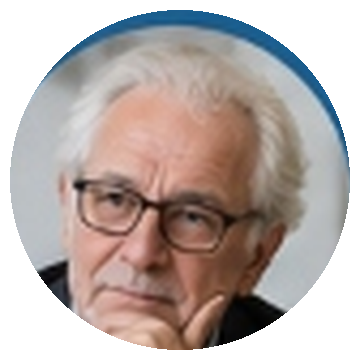
\includegraphics[width=2.06cm]{img_infografia/meirieu_photo.png}};

  \fill[infOrangeLight] (17.12,-3.04) rectangle (25.03,-2.56);
  \node[font=\fontsize{6.9}{8.0}\selectfont\bfseries\color{infOrange}] at (21.075,-2.80) {De la selección por prerrequisitos a «dar mejor»};

  \InfSectionBar{17.20}{-3.16}{infOrange}{infOrangeLight}{target}{Idea central del eje}
  \node[anchor=north west,text width=7.65cm,align=left,font=\fontsize{6.6}{8.0}\selectfont\color{infInk},inner sep=0pt] at (17.25,-3.74) {%
    Dejemos de convertir objetivos educativos en filtros de entrada. Ante la dificultad, la escuela justa ofrece «algo más» —rodeo didáctico— y abre un «mundo de tesoros» colaborativo.%
  };

  \InfSectionBar{17.20}{-4.86}{infOrange}{infOrangeLight}{key}{Conceptos clave}
  \InfConceptCard{17.20}{-5.44}{infOrange}{infOrangeCard}{balanza}{\textbf{Derecho vs. ocasión}\\Igualdad real de aprendizaje.}
  \InfConceptCard{19.17}{-5.44}{infOrange}{infOrangeCard}{target}{\textbf{Metas, no filtros}\\Entrenar antes de evaluar.}
  \InfConceptCard{21.14}{-5.44}{infOrange}{infOrangeCard}{andamio}{\textbf{«Algo más»}\\Rodeo frente a «más igual».}
  \InfConceptCard{23.11}{-5.44}{infOrange}{infOrangeCard}{lupa}{\textbf{Mundo de tesoros}\\Curiosidad frente a consumo.}

  \InfSectionBar{17.20}{-7.78}{infOrange}{infOrangeLight}{bulb}{Tesis principales}
  \InfBullet{17.22}{-8.38}{infOrange}{Rechazar el «síndrome del hospital» de la Carta a una profesora (Barbiana, 1967): no descartar a quien más apoyo requiere.}
  \InfBullet{17.22}{-9.04}{infOrange}{Aumentar dosis de idénticos ejercicios («más de lo mismo») profundiza el bloqueo; urge diagnóstico presencial.}
  \InfBullet{17.22}{-9.70}{infOrange}{Superar el taylorismo escolar y construir ecología sustantiva, no proyectos «suplemento de alma».}
  \InfBullet{17.22}{-10.36}{infOrange}{Sustituir un «mundo de tiendas» competitivo por un «mundo de tesoros» donde \textit{«nada se juega definitivamente»}.}

  \InfSectionBar{17.20}{-11.12}{infOrange}{infOrangeLight}{gear}{Implicaciones en Matemáticas}
  \InfCheck{17.22}{-11.72}{infOrange}{Cambiar representación verbal o gráfica cuando el despeje falla.}
  \InfCheck{17.22}{-12.26}{infOrange}{Valorar preguntas de diagnóstico sobre «matemáticas ingenuas».}
  \InfCheck{17.22}{-12.80}{infOrange}{Ofrecer segundas versiones tras retroalimentación formativa.}
  \InfCheck{17.22}{-13.34}{infOrange}{Conectar CONALEP, CECyTE e ingeniería con justicia educativa.}

  \fill[infOrangeLight,rounded corners=5pt] (17.20,-15.52) rectangle (24.95,-14.05);
  \node[text width=7.35cm,align=center,font=\fontsize{6.6}{8.1}\selectfont\color{infOrange}] at (21.075,-14.78) {%
    \textbf{\textit{«Porque nada, nunca, se juega definitivamente: todo estudiante tiene derecho a comprender.»}}\\
    {\scriptsize — Eje ético · Meirieu (2020)}%
  };

  % PIE DE FUENTE Y CREDITOS
  \draw[fill=infNavy,draw=infNavy,rounded corners=6pt] (0.0,-16.92) rectangle (25.15,-15.88);
  \node[inner sep=0pt] at (0.72,-16.40) {\InfIconOutline[0.36]{libro}{white}};
  \node[anchor=west,text width=16.8cm,align=left,font=\fontsize{6.6}{8.0}\selectfont\color{white}] at (1.30,-16.40) {%
    \textbf{FUENTE BASE (APA 7):} Meirieu, P. (2020, 18 de abril). \textit{«La escuela después»... ¿con la pedagogía de antes?} Movimiento Cooperativo de Escuela Popular (MCEP de Madrid; trad. de \textit{Café pédagogique}). \url{https://www.mcep.es/la-escuela-despues-con-la-pedagogia-de-antes-philippe-meirieu/}%
  };
  \node[anchor=east,text width=6.4cm,align=right,font=\fontsize{6.1}{7.4}\selectfont\color{white!90}] at (24.90,-16.40) {%
    \textbf{Mtro. Martín Jonathan de la Cruz Muñoz (Matrícula 00874)}\\
    IIIEPE · MAEM · Cohorte SD26 · Actividad 3 (Módulo 51440)%
  };
\end{tikzpicture}}
\end{frame}

\begin{frame}[plain]
  \centering
  \resizebox{0.97\textwidth}{!}{\begin{tikzpicture}[x=1cm,y=1cm]
  % Lienzo global 25.8cm x 17.1cm
  \fill[infPaper] (-0.30,-17.05) rectangle (25.45,0.20);

  % ============================================================================
  % COLUMNA 1: PHILIPPE MEIRIEU (2020) - AZUL MARINO (x = 0.0 .. 8.15)
  % ============================================================================
  \draw[fill=white,draw=infNavy,line width=1.1pt,rounded corners=7pt] (0.0,-15.72) rectangle (8.15,0.0);
  \fill[infNavy,rounded corners=6pt] (0.0,-2.48) rectangle (8.15,0.0);
  \fill[infNavy] (0.0,-2.48) rectangle (8.15,-2.00);
  \node[anchor=north west,text width=5.45cm,align=left,inner sep=0pt] at (0.28,-0.22) {%
    {\color{white}\fontsize{12.5}{14}\selectfont\bfseries Philippe Meirieu\par}\vspace{2pt}%
    {\color{white!90}\fontsize{7.4}{8.8}\selectfont\bfseries «La escuela después»... ¿con la\\pedagogía de antes?\par}\vspace{3pt}%
    {\colorbox{infBlueAccent}{\color{white}\fontsize{6.5}{7.5}\selectfont\bfseries\ 2020 · MCEP de Madrid \ }}%
  };
  \node[inner sep=0pt] at (6.92,-1.24) {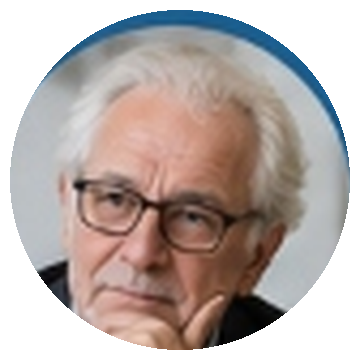
\includegraphics[width=2.06cm]{img_infografia/meirieu_photo.png}};

  % Cintillo subtitulo col 1
  \fill[infBlueLight] (0.12,-3.04) rectangle (8.03,-2.56);
  \node[font=\fontsize{7.0}{8.2}\selectfont\bfseries\color{infNavy}] at (4.075,-2.80) {Repensar la escuela para un mundo en transformación};

  % Idea central col 1
  \InfSectionBar{0.20}{-3.16}{infNavy}{infBlueLight}{target}{Idea central}
  \node[anchor=north west,text width=7.65cm,align=left,font=\fontsize{6.6}{8.0}\selectfont\color{infInk},inner sep=0pt] at (0.25,-3.74) {%
    La crisis puede ser oportunidad para transformar la educación, pero solo si cuestionamos las prácticas que reproducen desigualdad y devolvemos la pedagogía al centro.%
  };

  % Conceptos clave col 1 (4 tarjetas con pictogramas)
  \InfSectionBar{0.20}{-4.86}{infNavy}{infBlueLight}{key}{Conceptos clave}
  \InfConceptCard{0.20}{-5.44}{infNavy}{infBlueCard}{personas}{\textbf{Escuela como bien común}\\Espacio público de encuentro.}
  \InfConceptCard{2.17}{-5.44}{infNavy}{infBlueCard}{autonomia}{\textbf{Autonomía con sentido}\\Se construye con apoyo guiado.}
  \InfConceptCard{4.14}{-5.44}{infNavy}{infBlueCard}{dialogo}{\textbf{Cooperación y alteridad}\\Decir «yo» en un «nosotros».}
  \InfConceptCard{6.11}{-5.44}{infNavy}{infBlueCard}{alerta}{\textbf{Riesgos de retorno}\\Evitar volver a «lo anormal».}

  % Aportes principales col 1
  \InfSectionBar{0.20}{-7.78}{infNavy}{infBlueLight}{bulb}{Aportes principales}
  \InfBullet{0.22}{-8.38}{infNavy}{Formar ciudadanía libre, crítica y solidaria desde conocimientos «infinitamente compartibles» (Fichte).}
  \InfBullet{0.22}{-9.04}{infNavy}{Superar la selección sobre prerrequisitos: motivación y esfuerzo son metas, no filtros de exclusión.}
  \InfBullet{0.22}{-9.70}{infNavy}{Ofrecer «algo más» cara a cara cuando el alumno se bloquea en lugar de repetir «más de lo mismo».}
  \InfBullet{0.22}{-10.36}{infNavy}{La tecnología no sustituye la relación educativa; rechazar el conductismo individualista de pantalla.}

  % Implicaciones para la practica col 1
  \InfSectionBar{0.20}{-11.12}{infNavy}{infBlueLight}{gear}{Implicaciones para la práctica}
  \InfCheck{0.22}{-11.72}{infNavy}{Diseñar debates matemáticos que fomenten ayuda mutua.}
  \InfCheck{0.22}{-12.26}{infNavy}{Atender desigualdades materiales brindando andamiajes accesibles.}
  \InfCheck{0.22}{-12.80}{infNavy}{Evitar rutinas algorítmicas mecánicas sin reflexión conceptual.}
  \InfCheck{0.22}{-13.34}{infNavy}{Sostener una escuela incluyente donde cada estudiante tome la palabra.}

  % Tarjeta inferior col 1
  \fill[infBlueLight,rounded corners=5pt] (0.20,-15.52) rectangle (7.95,-14.05);
  \node[text width=7.35cm,align=center,font=\fontsize{6.6}{8.1}\selectfont\color{infNavy}] at (4.075,-14.78) {%
    \textbf{\textit{«Hacer escuela es hacer sociedad: enseñar la clase para que el mundo sea un mundo de tesoros.»}}\\
    {\scriptsize — Philippe Meirieu (2020)}%
  };

  % ============================================================================
  % COLUMNA 2: KEITH SAWYER (2008) - VERDE ESMERALDA (x = 8.50 .. 16.65)
  % ============================================================================
  \draw[fill=white,draw=infGreen,line width=1.1pt,rounded corners=7pt] (8.50,-15.72) rectangle (16.65,0.0);
  \fill[infGreen,rounded corners=6pt] (8.50,-2.48) rectangle (16.65,0.0);
  \fill[infGreen] (8.50,-2.48) rectangle (16.65,-2.00);
  \node[anchor=north west,text width=5.45cm,align=left,inner sep=0pt] at (8.78,-0.22) {%
    {\color{white}\fontsize{12.5}{14}\selectfont\bfseries Keith Sawyer\par}\vspace{2pt}%
    {\color{white!90}\fontsize{7.4}{8.8}\selectfont\bfseries Aportes de las ciencias del\\aprendizaje\par}\vspace{3pt}%
    {\colorbox{infGreenAccent}{\color{white}\fontsize{6.5}{7.5}\selectfont\bfseries\ 2008 · OECD / CERI \ }}%
  };
  \node[inner sep=0pt] at (15.42,-1.24) {
\includegraphics[width=2.06cm]{img_infografia/sawyer_photo.png}};

  \fill[infGreenLight] (8.62,-3.04) rectangle (16.53,-2.56);
  \node[font=\fontsize{7.0}{8.2}\selectfont\bfseries\color{infGreen}] at (12.575,-2.80) {Cómo aprendemos y qué pueden hacer las escuelas};

  \InfSectionBar{8.70}{-3.16}{infGreen}{infGreenLight}{target}{Idea central}
  \node[anchor=north west,text width=7.65cm,align=left,font=\fontsize{6.6}{8.0}\selectfont\color{infInk},inner sep=0pt] at (8.75,-3.74) {%
    El aprendizaje profundo ocurre cuando el estudiantado participa activamente en desafíos auténticos, articula su pensamiento y construye saber en interacción social y andamiada.%
  };

  \InfSectionBar{8.70}{-4.86}{infGreen}{infGreenLight}{key}{Conceptos clave}
  \InfConceptCard{8.70}{-5.44}{infGreen}{infGreenCard}{cerebro}{\textbf{Aprendizaje profundo}\\Comprensión y transferencia real.}
  \InfConceptCard{10.67}{-5.44}{infGreen}{infGreenCard}{construccion}{\textbf{Construcción activa}\\Partir de saberes previos.}
  \InfConceptCard{12.64}{-5.44}{infGreen}{infGreenCard}{dialogo}{\textbf{Interacción social}\\Conocimiento distribuido.}
  \InfConceptCard{14.61}{-5.44}{infGreen}{infGreenCard}{bulb}{\textbf{Creatividad aplicada}\\Analistas simbólicos críticos.}

  \InfSectionBar{8.70}{-7.78}{infGreen}{infGreenLight}{bulb}{Aportes principales}
  \InfBullet{8.72}{-8.38}{infGreen}{Superar el instruccionismo de la era industrial basado en transmisión memorística y pasos mecánicos.}
  \InfBullet{8.72}{-9.04}{infGreen}{Reconocer concepciones previas («matemáticas ingenuas») para reestructurar errores conceptuales.}
  \InfBullet{8.72}{-9.70}{infGreen}{Fomentar articulación oral y escrita, metacognición y andamiaje (\textit{scaffolding}) gradualmente retirado.}
  \InfBullet{8.72}{-10.36}{infGreen}{La evidencia TIMSS demuestra que mayor coherencia conceptual rinde más que currículos saturados.}

  \InfSectionBar{8.70}{-11.12}{infGreen}{infGreenLight}{gear}{Implicaciones para la práctica}
  \InfCheck{8.72}{-11.72}{infGreen}{Plantear retos de modelación ligados a prácticas profesionales.}
  \InfCheck{8.72}{-12.26}{infGreen}{Promover equipos con roles rotativos e interdependencia real.}
  \InfCheck{8.72}{-12.80}{infGreen}{Usar guías decrecientes sin resolver el ejercicio por el alumno.}
  \InfCheck{8.72}{-13.34}{infGreen}{Evaluar comprensión conceptual, coherencia y transferencia.}

  \fill[infGreenLight,rounded corners=5pt] (8.70,-15.52) rectangle (16.45,-14.05);
  \node[text width=7.35cm,align=center,font=\fontsize{6.6}{8.1}\selectfont\color{infGreen}] at (12.575,-14.78) {%
    \textbf{\textit{«Aprendemos mejor cuando externalizamos ideas, colaboramos en comunidad e integramos saberes.»}}\\
    {\scriptsize — R. Keith Sawyer (2008)}%
  };

  % ============================================================================
  % COLUMNA 3: FELIPE MARTÍNEZ RIZO (2026) - TERRACOTA (x = 17.00 .. 25.15)
  % ============================================================================
  \draw[fill=white,draw=infOrange,line width=1.1pt,rounded corners=7pt] (17.00,-15.72) rectangle (25.15,0.0);
  \fill[infOrange,rounded corners=6pt] (17.00,-2.48) rectangle (25.15,0.0);
  \fill[infOrange] (17.00,-2.48) rectangle (25.15,-2.00);
  \node[anchor=north west,text width=5.45cm,align=left,inner sep=0pt] at (17.28,-0.22) {%
    {\color{white}\fontsize{12.0}{14}\selectfont\bfseries Felipe Martínez Rizo\par}\vspace{2pt}%
    {\color{white!90}\fontsize{7.4}{8.8}\selectfont\bfseries Lectura contextualizada de\\PISA 2025\par}\vspace{3pt}%
    {\colorbox{infOrangeAccent}{\color{white}\fontsize{6.5}{7.5}\selectfont\bfseries\ 2026 · Distancia por tiempos \ }}%
  };
  \node[inner sep=0pt] at (23.92,-1.24) {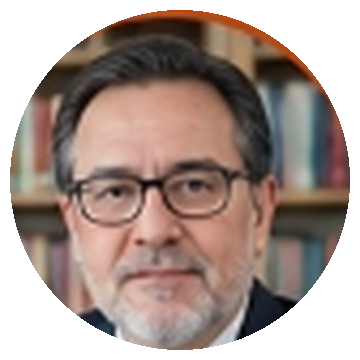
\includegraphics[width=2.06cm]{img_infografia/martinez_photo.png}};

  \fill[infOrangeLight] (17.12,-3.04) rectangle (25.03,-2.56);
  \node[font=\fontsize{7.0}{8.2}\selectfont\bfseries\color{infOrange}] at (21.075,-2.80) {Más allá del puntaje: comprender para mejorar};

  \InfSectionBar{17.20}{-3.16}{infOrange}{infOrangeLight}{target}{Idea central}
  \node[anchor=north west,text width=7.65cm,align=left,font=\fontsize{6.6}{8.0}\selectfont\color{infInk},inner sep=0pt] at (17.25,-3.74) {%
    Los resultados de PISA deben leerse desde su trayectoria histórica, cobertura escolar y contexto social: no son un ranking definitivo, sino insumo para políticas y prácticas justas.%
  };

  \InfSectionBar{17.20}{-4.86}{infOrange}{infOrangeLight}{key}{Conceptos clave}
  \InfConceptCard{17.20}{-5.44}{infOrange}{infOrangeCard}{grafica}{\textbf{Series y contexto}\\PISA 2018--2025 con cautela.}
  \InfConceptCard{19.17}{-5.44}{infOrange}{infOrangeCard}{balanza}{\textbf{Equidad e inclusión}\\Efecto de ampliación escolar.}
  \InfConceptCard{21.14}{-5.44}{infOrange}{infOrangeCard}{doc}{\textbf{Uso evaluativo}\\Orientar mejora, no castigo.}
  \InfConceptCard{23.11}{-5.44}{infOrange}{infOrangeCard}{lupa}{\textbf{Lectura crítica}\\Indagar causas multifactoriales.}

  \InfSectionBar{17.20}{-7.78}{infOrange}{infOrangeLight}{bulb}{Aportes principales}
  \InfBullet{17.22}{-8.38}{infOrange}{Registra descensos en México (lectura $420\to 415\to 408$; matemáticas $409\to 395\to 388$; ciencias $419\to 410\to 414$).}
  \InfBullet{17.22}{-9.04}{infOrange}{Advierte contra rankings alarmistas: comparar sistemas latinoamericanos afines aporta mayor rigor analítico.}
  \InfBullet{17.22}{-9.70}{infOrange}{El aprendizaje responde a factores escolares y extraescolares lentos; la correlación no sustituye explicación causal.}
  \InfBullet{17.22}{-10.36}{infOrange}{Urge reconstruir un sistema nacional propio e independiente que evalúe procesos de aula y escuelas eficaces.}

  \InfSectionBar{17.20}{-11.12}{infOrange}{infOrangeLight}{gear}{Implicaciones para la práctica}
  \InfCheck{17.22}{-11.72}{infOrange}{Usar diagnósticos locales para detectar rezagos comprensivos.}
  \InfCheck{17.22}{-12.26}{infOrange}{Evitar entrenar mecánicamente «para la prueba» estandarizada.}
  \InfCheck{17.22}{-12.80}{infOrange}{Considerar desigualdades de entorno, conectividad y jornada laboral.}
  \InfCheck{17.22}{-13.34}{infOrange}{Articular evaluación formativa cercana con seguimiento continuo.}

  \fill[infOrangeLight,rounded corners=5pt] (17.20,-15.52) rectangle (24.95,-14.05);
  \node[text width=7.35cm,align=center,font=\fontsize{6.6}{8.1}\selectfont\color{infOrange}] at (21.075,-14.78) {%
    \textbf{\textit{«Los datos adquieren sentido cuando se interpretan desde la realidad de las escuelas y las personas.»}}\\
    {\scriptsize — Felipe Martínez Rizo (2026)}%
  };

  % ============================================================================
  % CINTILLO INFERIOR INTEGRADOR + CREDITOS (y = -15.88 .. -16.92)
  % ============================================================================
  \draw[fill=infNavy,draw=infNavy,rounded corners=6pt] (0.0,-16.92) rectangle (25.15,-15.88);
  \node[inner sep=0pt] at (0.72,-16.40) {\InfIconOutline[0.36]{libro}{white}};
  \node[anchor=west,text width=16.8cm,align=left,font=\fontsize{7.4}{8.8}\selectfont\color{white}] at (1.30,-16.40) {%
    \textbf{Tres miradas, un mismo propósito:} una escuela más justa (Meirieu, 2020), con aprendizajes profundos (Sawyer, 2008) y decisiones evaluativas basadas en evidencia contextualizada (Martínez Rizo, 2026).%
  };
  \node[anchor=east,text width=6.4cm,align=right,font=\fontsize{6.1}{7.4}\selectfont\color{white!90}] at (24.90,-16.40) {%
    \textbf{Mtro. Martín Jonathan de la Cruz Muñoz (Matrícula 00874)}\\
    IIIEPE · MAEM · Cohorte SD26 · 19 de noviembre de 2026%
  };
\end{tikzpicture}}
\end{frame}

\begin{frame}{Núcleos Críticos de Philippe Meirieu (2020)}
  \begin{columns}[T]
    \column{0.48\textwidth}
      \begin{block}{1. Hacer el aula y saber compartible}
        \begin{itemize}\scriptsize
          \item Articular lo singular («yo») dentro de un colectivo («nosotros»).
          \item Ofrecer conocimientos «infinitamente compartibles» (Fichte).
          \item Superar el regreso acrítico a «lo anormal».
        \end{itemize}
      \end{block}
    \column{0.48\textwidth}
      \begin{block}{2. Derecho efectivo vs. prerrequisitos}
        \begin{itemize}\scriptsize
          \item Motivación y autonomía son metas, no filtros excluyentes.
          \item Ofrecer «algo más» cara a cara en vez de «más de lo mismo».
          \item Abrir un «mundo de tesoros» cooperativo.
        \end{itemize}
      \end{block}
  \end{columns}
\end{frame}

\begin{frame}{Articulación con Keith Sawyer (2008) y Felipe Martínez Rizo (2026)}
  \renewcommand{\arraystretch}{1.28}
  \scriptsize
  \begin{tabular}{p{3.0cm}p{5.0cm}p{5.4cm}}
    \toprule
    \textbf{Autor y escala} & \textbf{Problema central} & \textbf{Traducción en Matemáticas técnicas} \\
    \midrule
    Philippe Meirieu (2020) · Institución & Brecha discurso--práctica y selección injusta. & Comunidades de argumentación con apoyos reales en CONALEP/CECyTE. \\
    Keith Sawyer (2008) · Aula cognitiva & Instruccionismo superficial de fábrica. & Andamiaje, saberes previos («matemáticas ingenuas») y transferencia. \\
    Martínez Rizo (2026) · Sistema (PISA) & Rankings sin contexto histórico ni social. & Diagnóstico local de comprensión frente a entrenamiento mecánico. \\
    \bottomrule
  \end{tabular}
\end{frame}

\begin{frame}{Conclusiones y Referencias (APA 7)}
  \begin{itemize}\small
    \item La infografía vectorial en LaTeX/TikZ sintetiza la cohesión entre propósito público (Meirieu), cognición profunda (Sawyer) y evidencia evaluativa (Martínez Rizo).
    \item En matemáticas, el rigor disciplinar solo se democratiza acompañando las dificultades con rodeos didácticos pertinentes.
  \end{itemize}
  \vspace{0.3cm}
  \scriptsize
  \textbf{Referencias:} Martínez Rizo, F. (2026). \textit{Resultados de PISA 2025}. Nexos; Meirieu, P. (2020). \textit{MCEP}; Sawyer, R. K. (2008). \textit{Optimizing learning}. OECD; UNESCO (2015). \textit{Replantear la educación}.
\end{frame}

\end{document}
